\documentclass[11pt]{scrartcl}
\usepackage[utf8]{inputenc}
\usepackage{enumitem}
\usepackage{amsfonts}
\usepackage{bbm}
\usepackage{newtxmath}
%\usepackage[square]{natbib}
\usepackage{amsmath}
\usepackage{mathrsfs,bm}
\usepackage{graphicx,epstopdf,caption}
\usepackage{float,subcaption,setspace,booktabs,multirow,supertabular,lscape,threeparttable}
\usepackage{float,colortbl}
\usepackage{placeins}
\usepackage{indentfirst}
\usepackage{enumitem}
\setlength{\parindent}{0pt} %% noindent for the entire file % or add indent {2em}
\usepackage{geometry}
\geometry{left=0.8in,right=0.8in,top=1in,bottom=0.5in}
\usepackage[noblocks]{authblk}
\usepackage{lipsum}%% a garbage package you don't need except to create examples.
\usepackage{fancyhdr}
\usepackage[svgnames]{xcolor}
\usepackage{listings}
\usepackage{verbatim}
\usepackage[round, semicolon, sort]{natbib}
\setlength{\parindent}{2em}
\usepackage[font={footnotesize, it}]{caption}

\pagestyle{fancy}
\lhead{CSCI 5561}  % set your name here
\chead{\large\textbf{Homework 3 - Scene Recognition}}
\rhead{He Zhou (zhou1354@umn.edu)}
\renewcommand{\headrulewidth}{0.4pt}

\lstset{language=R,
	basicstyle=\small\ttfamily,
	stringstyle=\color{DarkGreen},
	otherkeywords={0,1,2,3,4,5,6,7,8,9},
	morekeywords={TRUE,FALSE},
	deletekeywords={data,frame,length,as,character},
	keywordstyle=\color{blue},
	commentstyle=\color{DarkGreen},
}
\usepackage{Sweave}
\graphicspath{{Figures/}}  % set the path of figures
\usepackage{blindtext}
\usepackage{scrextend}
\addtokomafont{labelinglabel}{\bfseries}
\usepackage{appendix}
\usepackage[linesnumbered,ruled,vlined]{algorithm2e}

\usepackage{algpseudocode}  
\usepackage{hyperref}
\hypersetup{
    colorlinks=true,
    linkcolor=blue,
    filecolor=blue,      
    urlcolor=blue,
    citecolor=cyan,
}

\newcommand{\cX}{\mathcal{X}}
\newcommand{\cR}{\mathcal{R}}
\newcommand{\cV}{\mathcal{V}}
\newcommand{\bw}{\mathbf{w}}

	

\begin{document}

\title{CSCI 5561}
\author{\Large Homework 3 -- Scene Recognition\\
	He Zhou}  %% set your name on the main page
%\date{\vspace{-5ex}}  % suppress the output of date
\maketitle

The scene classification dataset consists of $15$ scene categories including office, kitchen, forest and so on. The visual recognition system will compute a set of image representations (tiny image and bag-of-word visual vocabulary) and predict the category of each testing image using the classifiers ($k$-nearest neighbor and SVM).


\paragraph{\textbf{Tiny Image KNN Classification:}}
The Tiny Image approach uses the function \texttt{get\_tiny\_image} to resize each image to a small, fixed resolution using function \texttt{cv2.resize} and normalize the tiny image to having zero mean and unit length. Given the tiny image representations, the function \texttt{predict\_knn} uses a $k$-nearest neighbor classifier (\texttt{sklearn.neighbors.NearestNeighbors}) to predict the label of the testing data. The number of neighbors for label prediction  is set to be $k=10$ and label is predicted as the voted majority of the labels of those $10$ nearest  neighbors. Based on the predicted labels on the testing data, the function \texttt{classify\_knn\_tiny} returns a $15\times 15$ confusion matrix and the accuracy of the testing data prediction.

The visualization of confusion matrix is given in Figure (1a) and the accuracy of the prediction is  $0.222$. We can see that the tiny image representation is not a particularly good representation. This is because it discards all of the high frequency image content and is not especially invariant to spatial or brightness shifts. 

\begin{figure}[H]
	\captionsetup[subfigure]{labelformat=empty}
	\centering
	\subcaptionbox{(1a) Tiny image KNN classification with accuracy $0.222$}{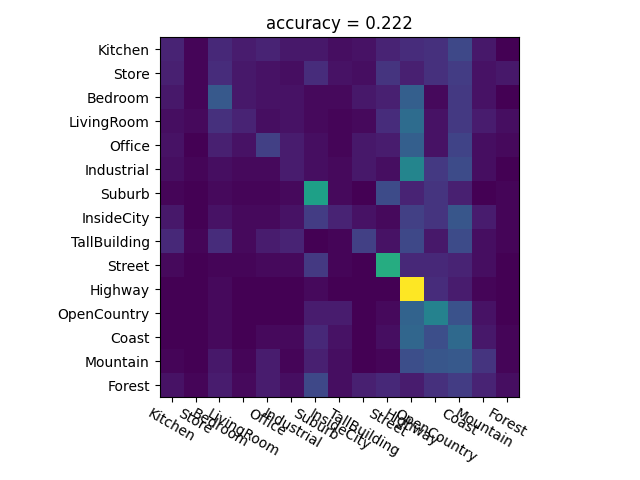
\includegraphics[height=6cm,keepaspectratio]{Tiny_KNN_confusion.jpg}}
	\subcaptionbox{(1b) Bag-of-word KNN classification with accuracy $0.515$}{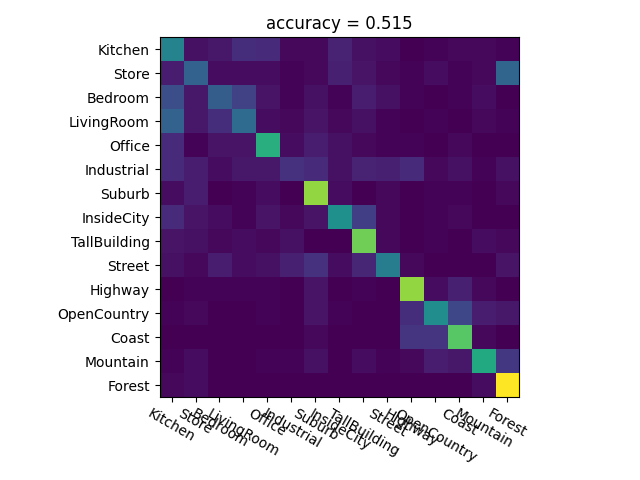
\includegraphics[height=6cm,keepaspectratio]{BoW_KNN_confusion.jpg}}
	\label{fig:confusion}
\end{figure}

\paragraph{\textbf{BoW $+$ KNN:}} 
The function \texttt{compute\_dsift} divides each image into small patches with both length and width equal to $\texttt{stride}=20$, and the keypoint for the sift descriptor is set to be the right botton corner of each small patch with keypoint diameter equals to $\texttt{size}=20$. Then this function returns a collection of sift features on the dense set of locations on image. Given the list of dense sift feature representation of training images, the function \texttt{build\_visual\_dictionary} builds a visual dictionary made of quantized SIFT features with $\texttt{dic\_size}=50$, in which the function $\texttt{sklearn.cluster.KMeans}(...,~\texttt{n\_init}=20,~\texttt{max\_iter}=300)$ is used to find the cluster centers. The output $\texttt{vocab}$ is saved in the file \texttt{`vacob\_knn\_bow.txt'}. In function \texttt{compute\_bow}, the bag-of-word (BoW) feature is constructed by counting SIFT features that fall into each cluster of the vocabulary, in which nearest neighbor with $\texttt{n\_neighbors}=1$ is used to find the closest cluster center.  Given the BoW features, the function \texttt{predict\_knn} again uses the $k$-nearest neighbor classifier with $k=10$  to predict the testing labels.

The visualization of confusion matrix is given in Figure (1b) and the accuracy of the prediction is  $0.515$. We can see that the BoW representation is a better representation. 

\paragraph{\textbf{BoW $+$ SVM}}
We use the BoW representation with $\texttt{stride}=15$ and $\texttt{size}=15$. The output $\texttt{vocab}$ is saved in the file \texttt{`vacob\_svm\_bow.txt'}. Given the BoW features, function \texttt{predict\_svm} uses a SVM classifier $\texttt{sklearn.svm.LinearSVC}$ to predict the label of the testing data. We train $15$ binary, 1-vs-all SVMs, where 1-vs-all means that each classifier will be trained to recognize `forest' vs `non-forest', `kitchen' vs `non-kitchen', etc. All $15$  binary SVM classifiers  are evaluated on each test  case and the classifier with the highest decision function score (given by \texttt{decision\_function}) wins. The free regularization parameter `lambda' is set to be $C=5$ to obtain good classification performance.

The visualization of confusion matrix is given in Figure (2) and the accuracy of the prediction is  $0.612$. We can see that the BoW representation with SVM classifier performs the best.


\begin{figure}[H]
	\captionsetup[subfigure]{labelformat=empty}
	\centering
	\subcaptionbox{(2) Bag-of-word SVM classification with accuracy $0.612$}{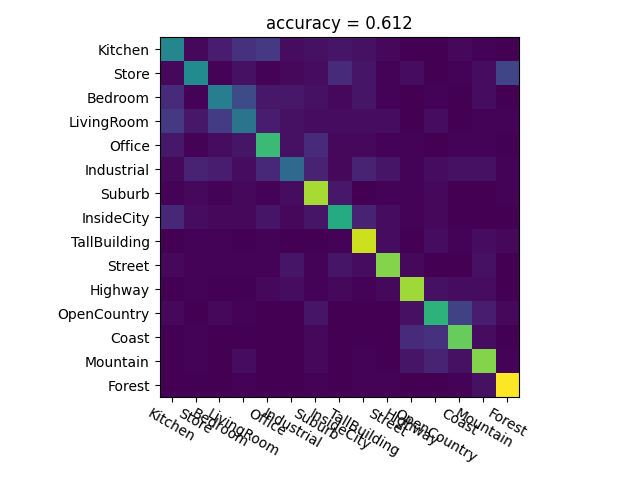
\includegraphics[height=7.5cm,keepaspectratio]{BoW_SVM_confusion.jpg}}
	\label{fig:confusion2}
\end{figure}













\nocite*{}  
%\bibliographystyle{apalike}  %disordered
%\bibliographystyle{plain}  %ordered by auther
%\bibliographystyle{unsrt}  %ordered as referenced
\bibliographystyle{IEEEtranN}
\bibliography{bibfile}






\end{document}